\documentclass[conference]{IEEEtran}
\IEEEoverridecommandlockouts
% The preceding line is only needed to identify funding in the first footnote. If that is unneeded, please comment it out.
\usepackage{cite}
\usepackage{amsmath,amssymb,amsfonts}
\usepackage{algorithmic}
\usepackage{graphicx}
\usepackage{textcomp}
\usepackage{graphicx}
\graphicspath{ {./images/} }
\usepackage{xcolor}
\usepackage[utf8]{inputenc}
\usepackage{hyperref}
\def\BibTeX{{\rm B\kern-.05em{\sc i\kern-.025em b}\kern-.08em
    T\kern-.1667em\lower.7ex\hbox{E}\kern-.125emX}}
\begin{document}

\title{
Sum of Geometric Progression Series \\
}

\author{\IEEEauthorblockN{Kalpana Khutela}
\IEEEauthorblockA{IIB2019019}
\and
\IEEEauthorblockN{Devang Bharti}
\IEEEauthorblockA{IIB2019020}
\and
\IEEEauthorblockN{Hitka}
\IEEEauthorblockA{IIB2019021}
}

\maketitle

\noindent \begin{abstract}

In this report we used divide and conquer approach to find the sum of Geometric Progression Series\\\\
Keyword : Geometric Progression, time complexity, space complexity,.

\end{abstract}


\section{\textbf{Introduction}}
\noindent In this problem, we have to find the sum of geometric progression series \\\\

\noindent For example: if we have n=5 and x=2, and as per question type of series is x,x2,x3,x4.... and so on. so common ratio will be x, so in above case it will be 2+4+8+16+32=62\\

\noindent we have given a brief idea of our algorithm \textbf{part II}.\\


\section{\textbf {Algorithm Approach}}

\begin{enumerate}

\item The algorithm asks for an integer ‘n’ as an input. which is stated as number of terms in that GP\\

\item Now the algorithm asks for a "X" value which will be the first term of that series.\\

\item Now we used the an application of divide and conquer approach named binary search to solve this problem.
\\
\item Call for the GeometricSequenceSum function with parameters as a(array) and n(size of array) which will give the answer \\
\item GeometricSequenceSum function is using a recursive approach to find the answer.\\
\item Base conditon:\\
Return 0 if size=0\\
else if size=1 then return a[0] element\\
\item Create two variables middle and rightSize.Initialize middle=size/2 and rightSize = size-middle.\\
\item Create two variables leftSum and rightSum.\\
\item Call for the GeometricSequenceSum function with parameters as a(array) and middle(size of array) which will return its computed sum in leftSum variable.\\
\item Call for the GeometricSequenceSum function with parameters as (a+ middle)(array passed from a+middle index) and rightSize(size of array) which will return its computed sum in rightSum variable.\\
\item After receiving values in leftSum and rightSum , these values are being added and final computed sum will be returned.\\
\item  Sum of the geometric sequence will be the required output and after  performing the above stated actions the requirement will be satisfied.\\




\textbf{For Example - }

Let input be
n=5 and x=2\\

array will be 2,4,8,16,32\\
now middle=2\\
right size=3\\\\
for left sum1\\
middle =1\\
right =1\\
for left sum1-2\\
size=1\\
so it will return a[0], that is 2\\
for left1 right sum1\\
size =1\\
it will return a[1], that is 4\\
and in final step we will have a[0]+a[1], that is 2+4=6\\\\

for right sum1\\
middle=1
right =2
for this middle it again go in function and size will be 1 so it will return a[2]\\
which is 8\\
and for right =2\\
middle =1\\
right =1\\
for this middle it again go in function and give a[3] that is 16\\
and for right it again go with size 1 and which will return a[4], that is 32\\
it will add 16,32,8 and give 56\\
which again called recursively and give 6+56, that is 62\\

\end{enumerate}

\section{\textbf{Pseudo Code}} 
\noindent Function GeometricSequenceSum \\
Pass : int arr[ ], int size\\
\begin{algorithmic}
    \STATE $base case$\\
	    \IF {$ size==0$}
	       return 0\\
            \ELSIF{$size==1$}
            return a[0]\\
            \ENDIF
        \ENDELSEIF
    \STATE $int middle=size/2$\\
    \STATE $int rightSize=size-middle$
    \STATE $int leftSum=GeometricSequenceSum(a,middle)$
    \STATE $int rightSum=GeometricSequenceSum(a+middle,rightSize)$
\end{algorithmic}

\section{\textbf {Time Complexity}}
\noindent The overall complexity of the question is O(n).
Our algorithm uses divide and conquer to find the sum of GP series.
\begin{figure}[htp]
    \centering
    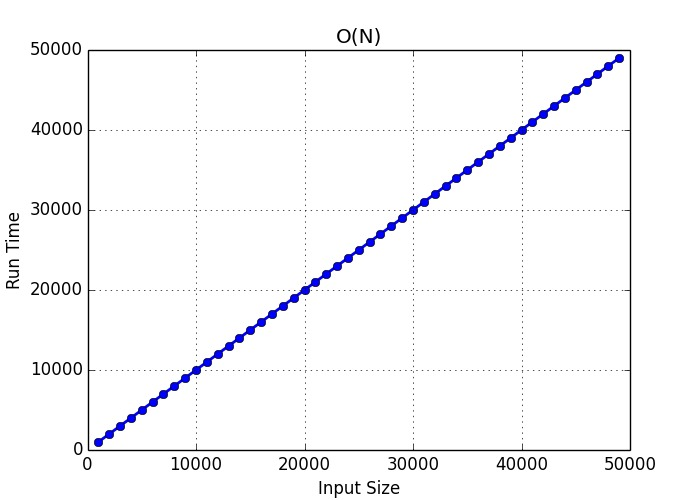
\includegraphics[width=8cm]{TimeComplexity}
    \caption{Time complexity curve}
    \label{fig:TimeComplexity.jpeg}
\end{figure}

\section{\textbf {Auxiliary Space Complexity}}
\noindent No extra space is used in this algorithm, so auxiliary space is constant.Only the input array is of size n.
Space Complexity = Input Space+Auxiliary Space, which is equal to O(n).


\begin{figure}[htp]
    \centering
    \includegraphics[width=8cm]{Aux_space}
    \caption{Auxiliary space complexity curve}
    \label{fig:Aux_space.jpeg}
\end{figure}

\section{\textbf {Conclusion}} \noindent The above proposed algorithm efficiently gives the sum of the given series. The algorithm proposed is very efficient both space and time wise with  O(n) time complexity.\\
\section{\textbf {References}} 
\begin{enumerate}

\item  \href{https://mathematics.laerd.com/maths/geometric-progression-intro.php}{Geometric Progression series and sum}\\
    
\item  \href{https://www.geeksforgeeks.org/divide-and-conquer-algorithm-introduction/}{
Divide and Conquer Algorithm | Introduction}
\\

\end{enumerate}

\end{document}